\section{\texorpdfstring{\WZ}{WZ} Background}
\label{sec:bkg_WZ}

This is the primary background in our search (about 51\,\%). To estimate this process, we define the \WZ control region by 3 leptons, an on-\Z OSSF pair, and $50\GeV < \MET < 100\GeV$. We use \WZ MC with fully leptonic decays and normalize the total number of events in the control region, after subtracting other backgrounds. The normalization factor is $0.95 \pm 0.07\stat$.

We validate the $n_\textrm{jets}$ distribution in the control region (Fig.~\ref{fig:WZ/NGOODJETS}) and find that $n_\textrm{jets}$ weights do not need to be applied. The \WZ-specific shape of the transverse mass distribution (Fig.~\ref{fig:WZ/MET50to100_MT}) is checked as well, where the transverse mass $M_\textrm{T}$ is defined as
$$M_\textrm{T} = \sqrt{2 \MET p_\textrm{T}^\ell \left( 1 - \cos\measuredangle(\vec E_\textrm{T}^\text{miss}, \vec p_\textrm{T}^{\,\ell}) \right)},$$ and $\ell$ refers to the lepton that is not part of the OSSF pair. In case of ambiguity, the OSSF pair is defined as the one whose invariant mass is closer to the \Z boson mass.

\begin{figure}
\begin{center}
	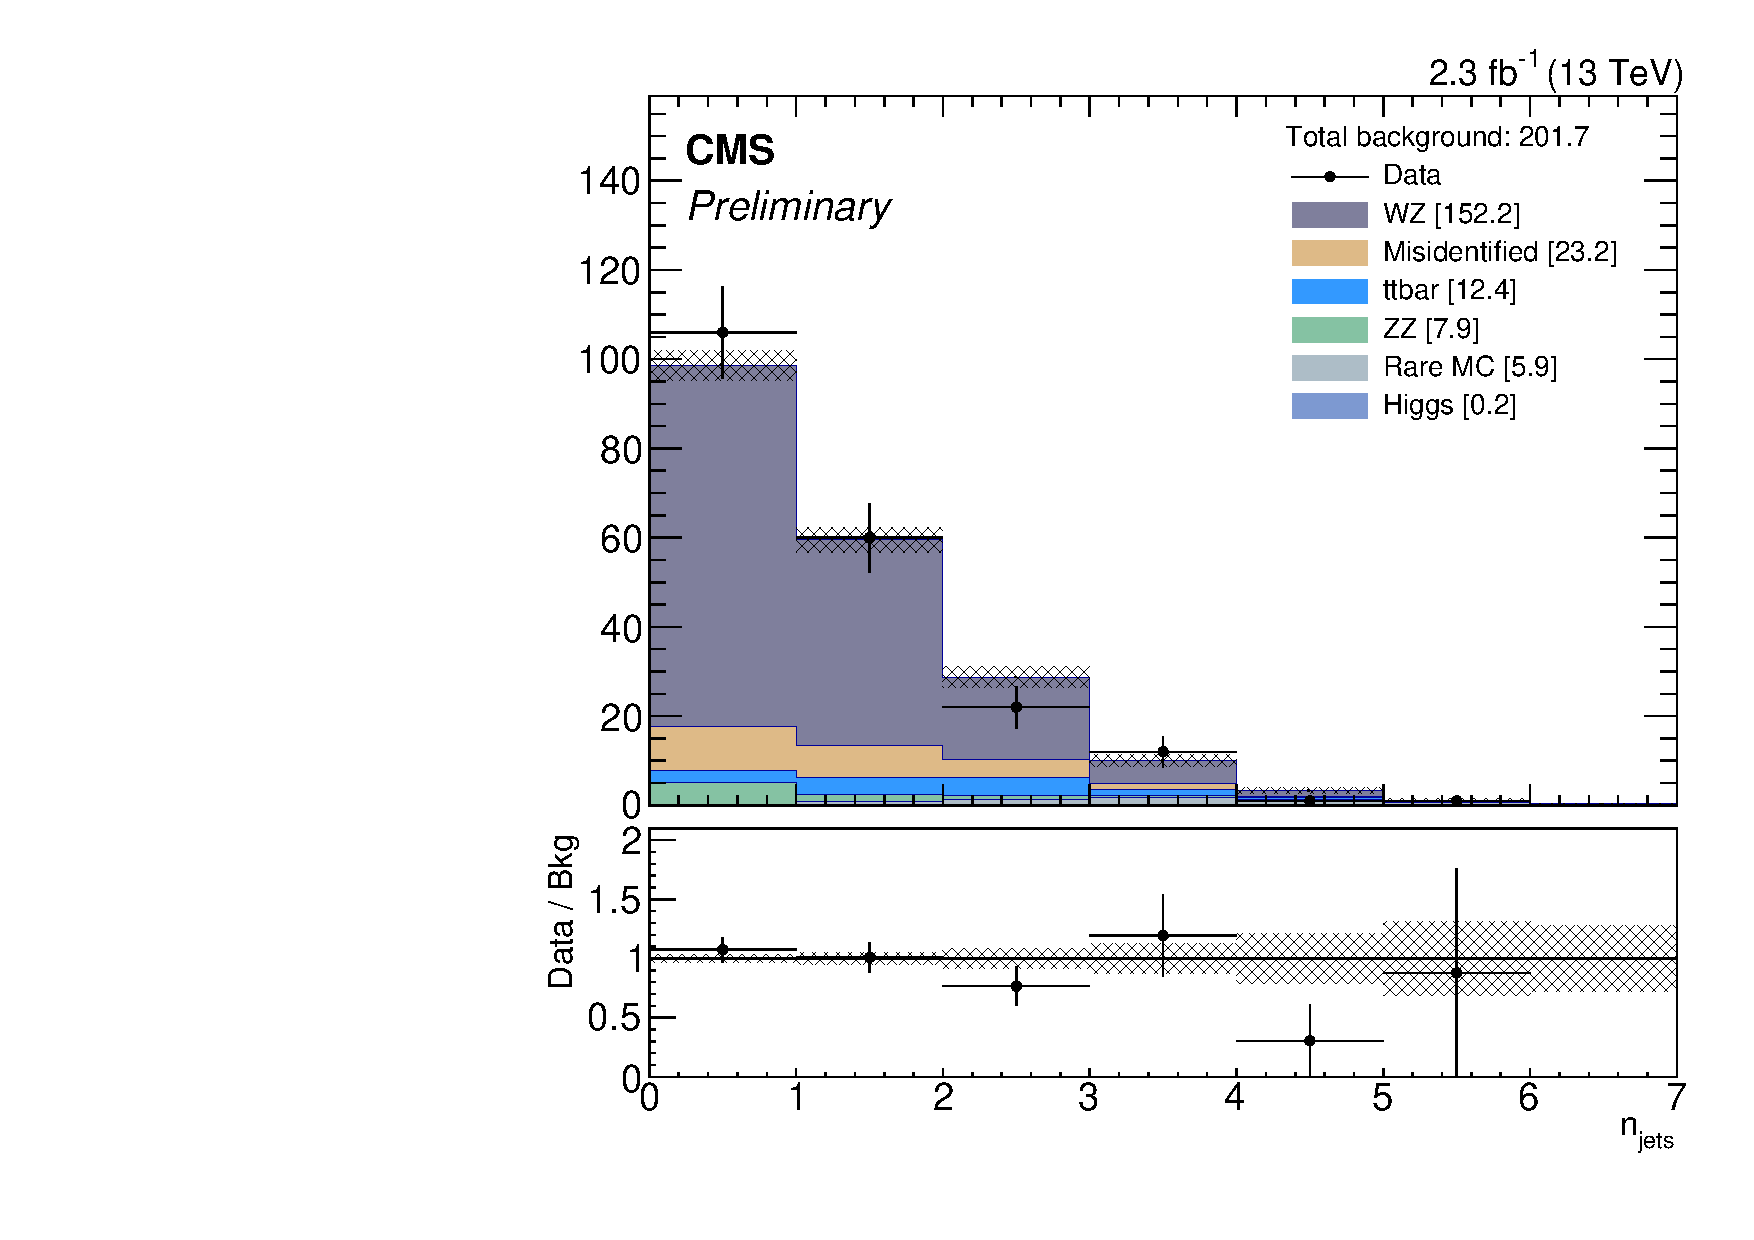
\includegraphics[width=.7\textwidth]{Background/bkg_WZ/WZ_MET50to100_NGOODJETS}
	\caption{$n_\textrm{jets}$ distribution in the \WZ-dominated control region (last bin includes overflow). Uncertainty bands include both statistical and systematic uncertainties, with the exception of the \WZ normalization uncertainty. \fixme{label}
	\label{fig:WZ/NGOODJETS}}
\end{center}
\end{figure}

\begin{figure}
\begin{center}
	\begin{subfigure}[b]{.7\textwidth}
		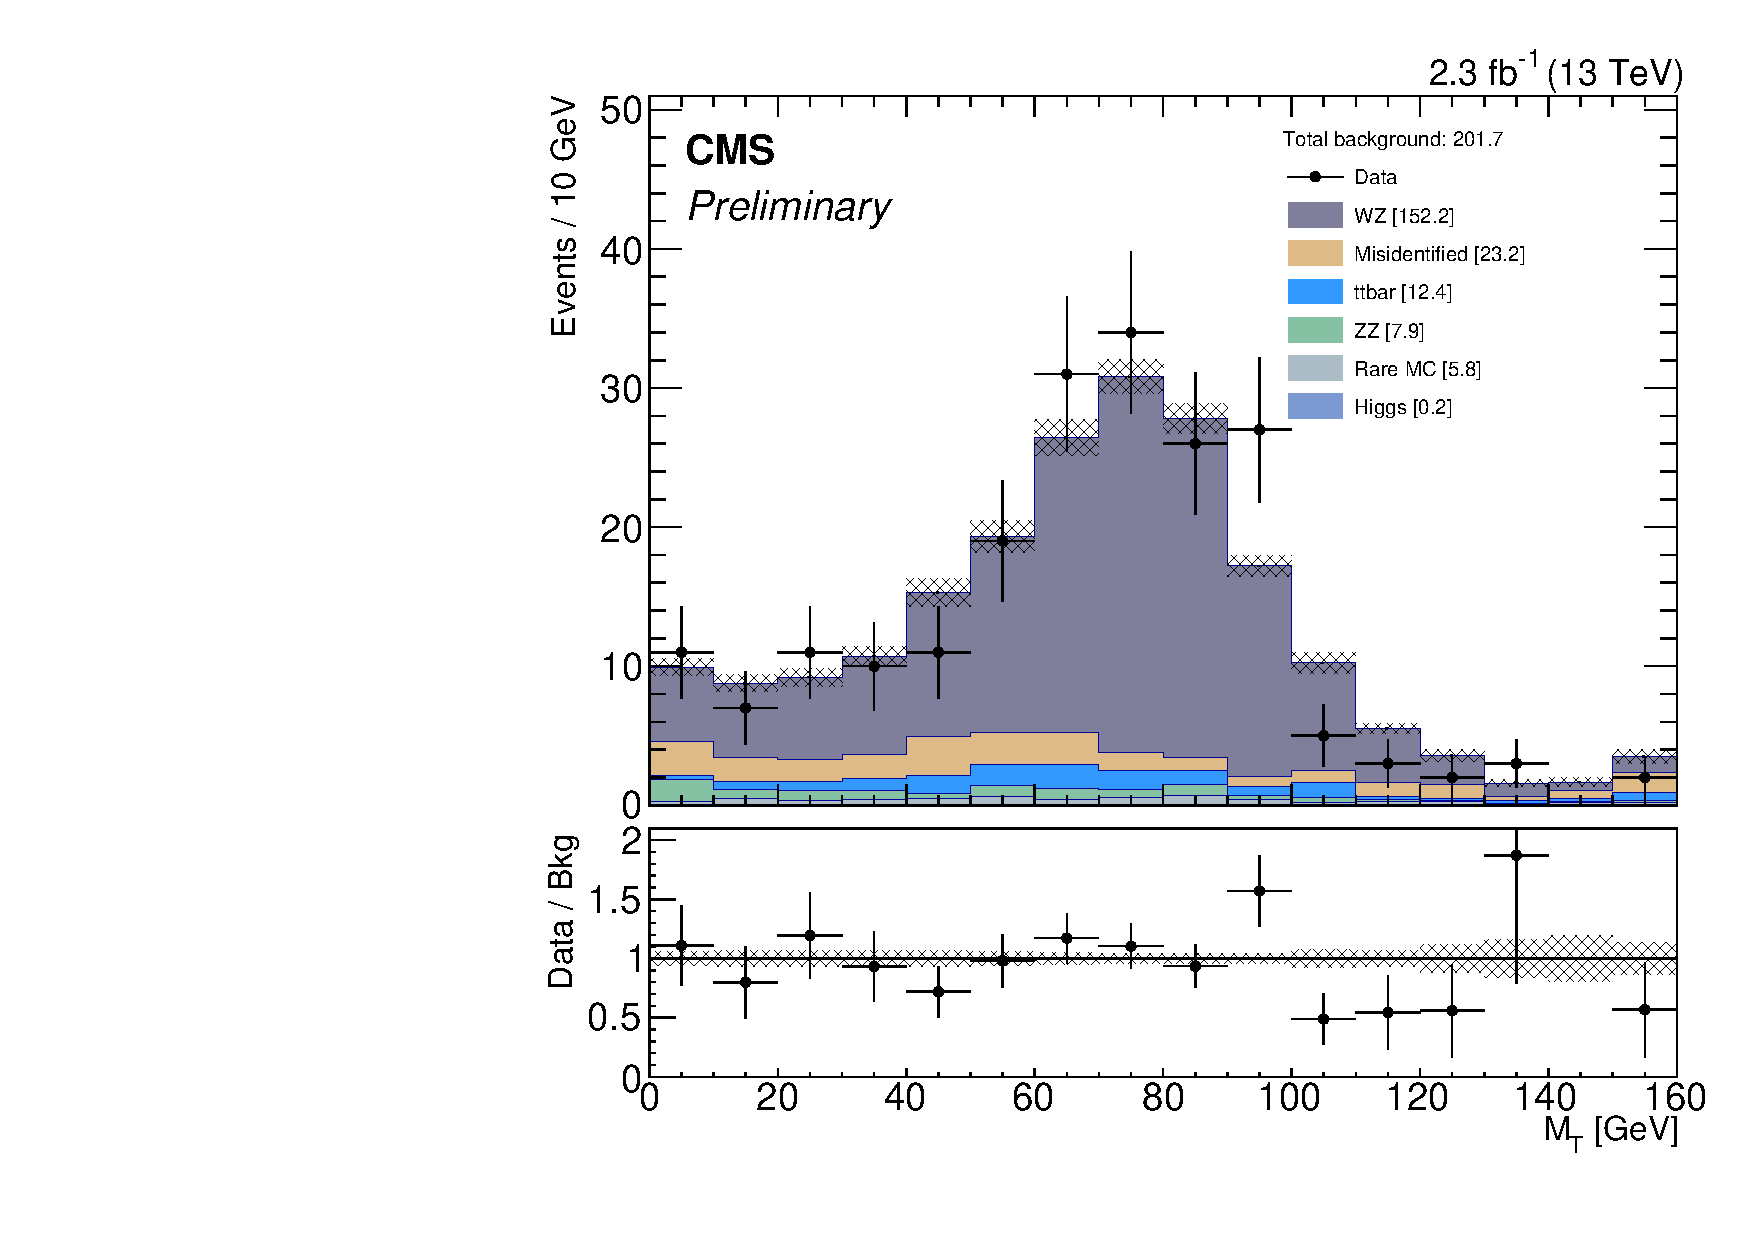
\includegraphics[width=\textwidth]{Background/bkg_WZ/WZ_MET50to100_MT}
		\caption{$50\GeV < \MET < 100\GeV$} \label{fig:WZ/MET50to100_MT}
	\end{subfigure}
	\begin{subfigure}[b]{.7\textwidth}
		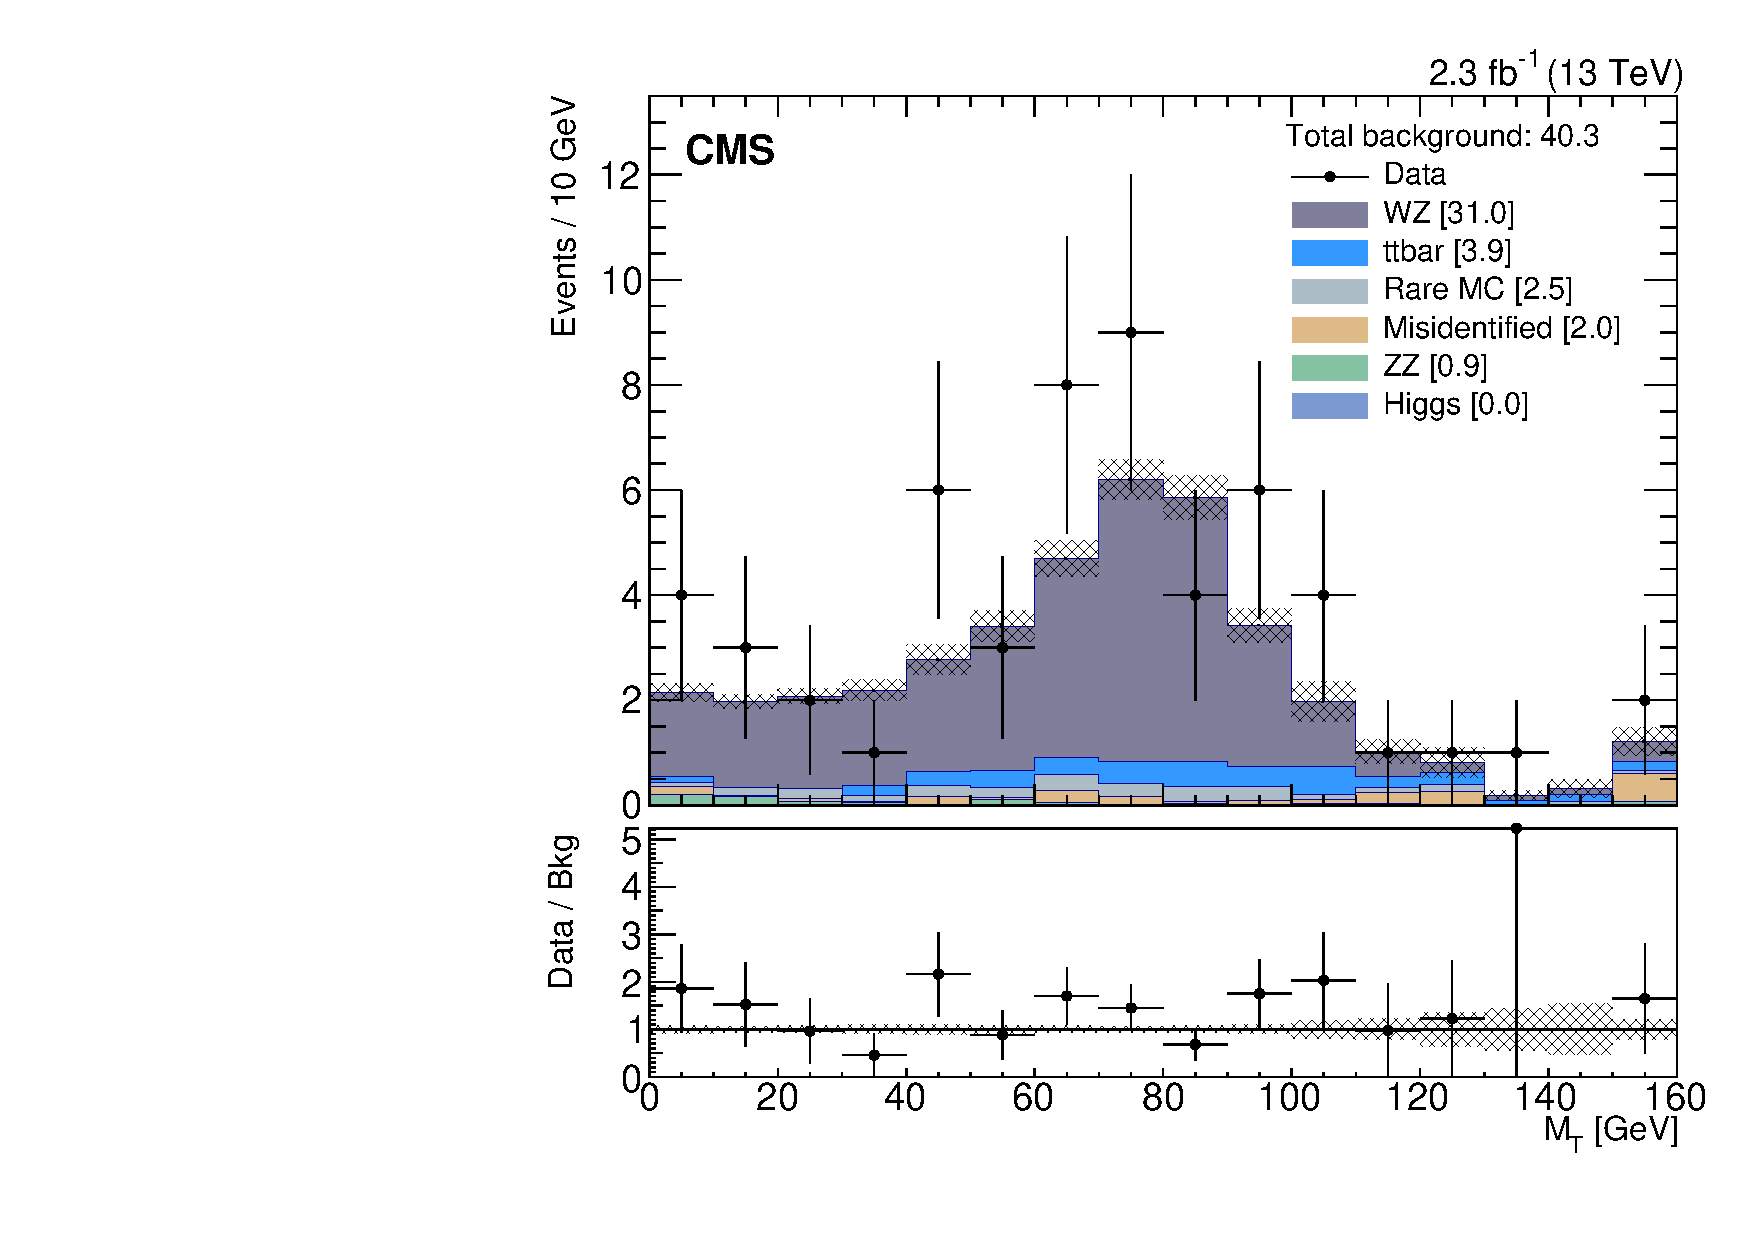
\includegraphics[width=\textwidth]{Background/bkg_WZ/WZ_MET100to150_MT}
		\caption{$100\GeV < \MET < 150\GeV$ \fixme{label}} \label{fig:WZ/MET100to150_MT}
	\end{subfigure}
	\caption{$M_\textrm{T}$ distributions in the \WZ-dominated control and validation regions (last bin includes overflow). Uncertainty bands include both statistical and systematic uncertainties, with the exception of the \WZ normalization uncertainty.
	\label{fig:WZ}}
\end{center}
\end{figure}

In the adjoining $100\GeV < \MET < 150\GeV$ validation region, we find that the normalization is off. Based on the amount of data investigated, we cannot tell whether this is a statistical fluctuation or a mismodeling effect. Detailed investigations of the extra events did not uncover any unexpected kinematic patterns. We thus assign a systematic uncertainty of 50\,\% based on the variation of the normalization factor between the normalization region and the validation region (see Fig.~\ref{fig:WZ/MET100to150_MT}).
